\documentclass{article}
\usepackage[utf8]{inputenc}
\usepackage{tikz}
\usepackage{amsmath}
\usepackage{graphicx}

\title{CS 460 Lab 1}
\author{Brian Rasmussen}
\date{September 2019}

\begin{document}

\maketitle

\section{Introduction}
This report dives into different experiments ran on simulated networks.
Experiments in part 1A were ran for different transmission and different propagation delay.
And experiments in part 1B were ran experimenting with the link utilization.
This report shows how each one of the listed parameters above effect the overall network.
\section{Two Nodes}
The following Scenario were used for testing.
\subsection{Scenario-1}
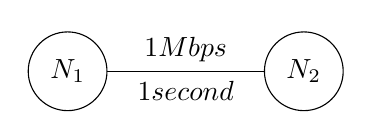
\begin{tikzpicture}
\draw (0,0) circle (.5cm)  node {$N_1$};
\draw (.5,0) -- (2.5,0) node[pos=.5,above] {$1Mbps$} node[pos=.5,below] {$1second$};
\draw (3,0) circle (.5cm) node {$N_2$};
\end{tikzpicture}
\begin{verbatim}
n1 n2
n2 n1

n1 n2 1Mbps 1seconds
n2 n1 1Mbps 1seconds
\end{verbatim}
\subsection{Simulation-1}
\begin{verbatim}
1 0 1.008
\end{verbatim}
\subsection{Math-Calculation-1}
\begin{equation}
    % Receive Time = BeginTime + Packet_{size}/d_{prop}
    Receive Time = StartTime + \frac {L}{R} + D_{prop}
\end{equation} 
\begin{equation}
    % Receive Time = BeginTime + Packet_{size}/d_{prop}
    1.008 = 0_{Sec} + \frac {8000_{bits}}{1000000_{bits per second}} + 1_{Sec}
\end{equation}
\subsection{Scenario-2}
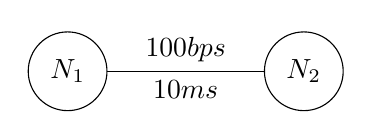
\begin{tikzpicture}
\draw (0,0) circle (.5cm)  node {$N_1$};
\draw (.5,0) -- (2.5,0) node[pos=.5,above] {$100bps$} node[pos=.5,below] {$10ms$};
\draw (3,0) circle (.5cm) node {$N_2$};
\end{tikzpicture}
\begin{verbatim}
n1 n2
n2 n1

n1 n2 100bps 10ms
n2 n1 100bps 10ms
\end{verbatim}
\subsection{Simulation-2}
\begin{verbatim}
1 0 80.01
\end{verbatim}
\subsection{Math-Calculation-2}
\begin{equation}
    % Receive Time = BeginTime + Packet_{size}/d_{prop}
    80.01 = 0_{Sec} + \frac {8000_{bits}}{100_{bits per second}} + .01_{Sec}
\end{equation}
\subsection{Scenario-3}
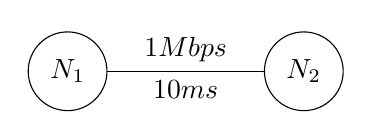
\begin{tikzpicture}
\draw (0,0) circle (.5cm)  node {$N_1$};
\draw (.5,0) -- (2.5,0) node[pos=.5,above] {$1Mbps$} node[pos=.5,below] {$10ms$};
\draw (3,0) circle (.5cm) node {$N_2$};
\end{tikzpicture}
\begin{verbatim}
n1 n2
n2 n1

n1 n2 1Mbps 10ms
n2 n1 1Mbps 10ms
\end{verbatim}
\subsection{Simulation-3}
\begin{verbatim}
1 0 0.018
2 0 0.026
3 0 0.034
4 2.0 2.018
\end{verbatim}
\subsection{Math-Calculation-3}
\begin{equation}
    % Receive Time = BeginTime + Packet_{size}/d_{prop}
    Receive Time = StartTime + \frac {L}{R} *(PacketNumber) + D_{prop} 
\end{equation} 
\begin{equation}
    % Receive Time = BeginTime + Packet_{size}/d_{prop}
    0.018 = 0_{Sec} + \frac {8000_{bits}}{1000000_{bits per second}} * (1) + .01_{Sec}
\end{equation}
\begin{equation}
    % Receive Time = BeginTime + Packet_{size}/d_{prop}
    0.026 = 0_{Sec} + \frac {8000_{bits}}{1000000_{bits per second}} * (2) + .01_{Sec}
\end{equation}
\begin{equation}
    % Receive Time = BeginTime + Packet_{size}/d_{prop}
    0.034 = 0_{Sec} + \frac {8000_{bits}}{1000000_{bits per second}} * (3) + .01_{Sec}
\end{equation}
\begin{equation}
    % Receive Time = BeginTime + Packet_{size}/d_{prop}
    2.018 = 2_{Sec} + \frac {8000_{bits}}{1000000_{bits per second}} * (1) + .01_{Sec}
\end{equation} 
\section{Three Nodes}
\subsection{Scenario-1}
\begin{verbatim}
a b
b a
b c
c b

a b 1Mbps 100ms
b a 1Mbps 100ms
b c 1Mbps 100ms
c b 1Mbps 100ms
\end{verbatim}
\subsection{Simulation-1}
\begin{verbatim}
996 7.96 8.176 0.216 0.016 0.2 6.2172489379e-15
997 7.968 8.184 0.216 0.016 0.2 6.2172489379e-15
998 7.976 8.192 0.216 0.016 0.2 6.2172489379e-15
999 7.984 8.2 0.216 0.016 0.2 6.2172489379e-15
1000 7.992 8.208 0.216 0.016 0.2 6.2172489379e-15
\end{verbatim}
\subsection{Math-1}
\begin{equation}
    8.208 = 2 * (\frac{8000_{bits}}{1Million_{bitpersec}}) + 2*0.1_{sec} + (Packet Number - 1) * (\frac{8000_{bits}}{1Million_{bitpersec}}) 
\end{equation}
\subsection{Scenario-2}
\begin{verbatim}
a b
b a
b c
c b

a b 1Gbps 100ms
b a 1Gbps 100ms
b c 1Gbps 100ms
c b 1Gbps 100ms
\end{verbatim}
\subsection{Simulation-2}
\begin{verbatim}
996 0.00796 0.207976 0.200016 1.6e-05 0.2 1.30104260698e-16
997 0.007968 0.207984 0.200016 1.6e-05 0.2 1.30104260698e-16
998 0.007976 0.207992 0.200016 1.6e-05 0.2 1.28369537222e-16
999 0.007984 0.208 0.200016 1.6e-05 0.2 1.28369537222e-16
1000 0.007992 0.208008 0.200016 1.6e-05 0.2 1.28369537222e-16
\end{verbatim}
\subsection{Math-2}
\begin{equation}
    .208008 = 2 * (\frac{8000_{bits}}{1Billion_{bitpersec}}) + 2*0.1_{sec} + (1000_{PacketNumber} - 1) * (\frac{8000_{bits}}{1Billion_{bitpersec}})
\end{equation}
\subsection{Scenario-2}
\begin{verbatim}
a b
b a
b c
c b

a b 1Mbps 100ms
b a 1Mbps 100ms
b c 256Kbps 100ms
c b 256Kbps 100ms
\end{verbatim}
\subsection{Simulation-3}
\begin{verbatim}
996 7.96 31.333 23.373 0.03925 0.2 23.13375
997 7.968 31.36425 23.39625 0.03925 0.2 23.157
998 7.976 31.3955 23.4195 0.03925 0.2 23.18025
999 7.984 31.42675 23.44275 0.03925 0.2 23.2035
1000 7.992 31.458 23.466 0.03925 0.2 23.22675
\end{verbatim}
\subsection{Math-3}
\begin{equation}
    31.458 = \frac {8000_{bits}}{1Million_{bitspersec}} + .1_{secs} + \frac{8000_{bits}}{256000_{bitspersec}} + .1_{secs} + (1000_{PacketNumber}-1) * \frac {8000_{bits}}{256000_{bitspersec}}
\end{equation}
\section{Qeueuing Theory}
\subsection{Network Configuration}
\begin{verbatim}
a b
b a
b c
c b

a b 1Mbps 100ms
b a 1Mbps 100ms
b c 1Mbps 100ms
c b 1Mbps 100ms
\end{verbatim}
\subsection{Experiment Process}
In order to send to measure the effect of the arrival rate.
We tried varying link utilization or ${p}$.
The ${p}$ values ranged from .1 to .98.
For each ${p}$ value we ran simulated sending packets for 10 minutes or 600 seconds.
When each packet was received we recorded the time received and the queuing delay.
Then by taking the average queuing delay we were able to graph queuing delay as a function of p.
\begin{figure}[htp]
    \centering
    \includegraphics[width=\textwidth]{delay.eps}
    \caption{Theoretical and Simulated delay}
    \label{fig:graph}
\end{figure}
\subsection{Discussion}
This actual results are very similar to the predicted.
There is some small variation but that is likely due to the exponential distribution of sending of the packets.
It is interesting to note that both the theoretical and the simulated queuing delay aren't to high until ${p > .9}$.
\subsection{Conclusion}
The result were pretty much as expected.
In the first part of the lab the bottle neck of the network was always what had a big influence on the total time.
That being transmission rate or the bandwidth.
Doing the first part of the project definitely cemented the interaction between different parts of the network.
In part it was interesting to look at queuing delay.
Even thought the queuing delay was exponential it didn't seem to bad until $p>.9$ which was higher then I thought it was going to be.
\end{document}
